\chapter{Sample Problem}
\label{chapter:sample-problem}

In order to validate the different modules of \texttt{hIPPYfire}, one of \texttt{hIPPYlib}'s Bayesian inversion test cases, namely \texttt{3-SubsurfaceBayesian} \cite{Villa_hIPPYlib_An_Extensible_2020}, was recreated. This test case utilized all of \texttt{hIPPYfire}'s models that have been currently developed. Additional test cases shall be added for future functionality. The test case is briefly discussed below; a detailed description of the test case can be found in \texttt{hIPPYlib}'s repository \cite{Villa_hIPPYlib_An_Extensible_2020}.

The objective of this test case is to compute the uncertainty in the solution of an inverse problem governed by an elliptic PDE via the Bayesian inference framework. However, this test case only solves the forward problem and computes the MAP point, as described in Section \ref{chapter: inverse-problems}. Please note that the following test case admits discretized expressions of the parameter space, i.e., they are finite-dimensional.

The objective of this sample problem is to compute the log coefficient field \textit{m} for an elliptic PDE with continuous state observations. In addition to the mesh set-up parameters (such as the dimension, mesh divisions, function space, etc), the user is required to provide the weak form of the PDE and the corresponding boundary conditions for forward and adjoint problems. The weak form of the PDE is given as follows:
\begin{equation}
    \label{eqn:pde}
    \begin{split}
    e^{m}\langle{\nabla{u}, \nabla{p}}\rangle = \langle{f, p}\rangle \textrm{ in } \Omega, \\
    u(\textbf{x}, \textbf{y}) = \textbf{y} \textrm{ on } \Gamma_D = \Gamma_{bottom} \bigcup \Gamma_{top}
    \end{split}
\end{equation}
where $\Omega = (0, 1) \times (0, 1)$ and $\Gamma_D$ is the union of the top and bottom boundaries of $\Omega$. $u$ is the state variable, $f \in \mathcal{L}^2(\Omega)$ is a source term (that is equated to zero in the current case), and $\langle{.,.}\rangle$ represents the standard inner product on $\mathcal{L}^2(\Omega)$. The spaces $V_{y}$ and $V_0$ are defined as follows:
$$
    V_y = \left\{ v \in H^1(\Omega) \textrm{ s.t. } v = \textbf{y} \textrm{ on } \Gamma_D \right\}
$$
$$
    V_0 = \left\{ v \in H^1(\Omega) \textrm{ s.t. } v = 0 \textrm{ on } \Gamma_D \right\}
$$
where $H^1(\Omega)$ is the Sobolev space whose derivatives are in $\mathcal{L}^2(\Omega)$. In the weak form of the PDE (Eqn. \ref{eqn:pde}), we attempt to find $u \in V_y$ using the test function $p \in V_0$.

The prior is a Gaussian distribution $\mathcal{N}(m_{pr}, C_{prior})$ s.t. $C_{prior} = \mathcal{A}^{-2}$, as shown in \cite{stuart2010inverse}. $\mathcal{A}$ is a differential operator with a domain $H^1({\Omega})$ and action as given below:

\begin{equation}
\label{eqn: prior_action}
 \left\{
    \begin{array}{lr}
        -\gamma\nabla.(\Theta\nabla{m}) + \delta{m} &  \textrm{ in } \Omega\\
        \Theta\nabla{m}.\textbf{n} + \beta{m} & \textrm{ in } \partial\Omega
    \end{array}
\right\}
\end{equation}

$\beta \propto \sqrt{\gamma\delta}$ is the optimal robin coefficient \cite{daon2016mitigating} to minimize boundary artifcats. $\Theta$ is an s.p.d anisotropic tensor of the form:

\begin{equation}
\label{eqn: Theta}
 \left\{
    \begin{array}{lr}
        \theta_1sin(\alpha)^2 &  (\theta_1 - \theta_2)sin(\alpha)cos(\alpha)\\
        (\theta_1 - \theta_2)sin(\alpha)cos(\alpha) & \theta_2cos(\alpha)^2
    \end{array}
\right\}
\end{equation}

The prior is chosen such that the well-posedness of this problem is ensured.

The log-likelihood (data misfit) functional is specfiied next. The noisy continuous data observations, $\textbf{d}$, are approximated s.t. $\textbf{d} \in \mathbb{R}^q$. They represent the observations of the state \textit{u} at $q = 16641$ random locations uniformly distributed in $\Omega$ 

\hl{@Umberto, kindly request you to verify the above statement. This is the reason why we have points in the RHS of the observations graph, even though it is a continuous state observation. \texttt{misfit.d} is initialized as \texttt{pde.generate\_state()} vector. If my explanation above is incorrect, could you please assist me in rectifying it? Thank you.}

\begin{equation}
    d = \mathcal{B}u + \eta
\end{equation}
where $\mathcal{B} : V_y \rightarrow \mathbb{R}^q$ is a linear observation operator. $\eta$ represents the noise vector and is a multivariate Gaussian variable with a distribution $\mathcal{N}(0, \Gamma_{noise})$ s.t. $\Gamma_{noise} = \sigma^2\textbf{I}$, where $\sigma = 0.01$ and $\textbf{I} = \mathbb{R}^{q \times q}$

The likelihood is then computed as follows:

\begin{equation}
    \pi_{like}(\textbf{d} | \textbf{m}) = exp(-\frac{1}{2}(\mathcal{B}u(m) -\textbf{d})^T\Gamma^{-1}_{noise}(\mathcal{B}u(m) -\textbf{d}))
\end{equation}

where $m_{pr}$ is the prior mean of the log coefficient field $m$. The above equation presents a discretized version of the likelihood function. The mean of the posterior distribution, also referred to as \textbf{${m_{MAP}} $}, is the parameter vector that maximizes the posterior. It is computed by solving the following variational non-linear least squares optimization problem:
\begin{equation}
    \textbf{m}_{MAP} := \underset{m \in H^1(\Omega)}{arg min}\mathcal{J}(\textbf{m}) := (\frac{1}{2} || \mathcal{B}u(m) - \textbf{d} ||^2_{\Gamma_{noise}^{-1}} + \frac{1}{2}|| \textbf{m} - \textbf{m}_{prior} || ^2_{C_{prior}^{-1}}
\end{equation}

This optimization problem has been solved using the inexact Newton-CG algorithm, which has been described in Appendix A of Villa et al. \cite{Villa_hIPPYlib_An_Extensible_2020}.

\hl{@Umberto, Since we do not go beyond the calculation of the MAP point, I have not included any more equations. Would you like me to include the Gradient and Hessian actions of the cost functional as well? Please let me know, and I shall include them appropriately. Although I might need your help in writing those since we only have the weak form of the PDE.}

The problem flow demonstrated above is represented through a few code snippets below.

\begin{itemize}
    \item \textbf{Mesh and FEM setup}: A two-dimensional unit square mesh is created with a P2 finite element space for \texttt{state} and \texttt{adjoint} variables and P1 for \texttt{parameter}.
    \begin{lstlisting}[language=python]
        ndim = 2
        nx = 64
        ny = 64
        mesh = fd.UnitSquareMesh(nx, ny)
        Vh2 = fd.FunctionSpace(mesh, 'Lagrange', 2)
        Vh1 = fd.FunctionSpace(mesh, 'Lagrange', 1)
        Vh = [Vh2, Vh1, Vh2]
    \end{lstlisting}
    \item \textbf{Forward Problem}: As mentioned in Section \ref{chapter: software}, the \texttt{PDEVariationalProblem} class sets up the forward problem component of the \textit{p2o} map. In addition to the finite element components defined above, it requires an expression of the weak form of the PDE (given by \texttt{pde\_varf}) and boundary conditions for the forward (\texttt{bc}) and incremental and adjoint problems (\texttt{bc0}).
    The \texttt{PDEVariationalProblem} class solves the forward/adjoint and incremental problems and computes the relevant partial derivatives with respect to the state, parameter, and adjoint variables.
    \begin{lstlisting}[language=python]
        u_bdr = fd.SpatialCoordinate(mesh)[1]
        u_bdr0 = fd.Constant(0.0)

        bc = fd.DirichletBC(Vh[STATE], u_bdr, [3, 4]) # [3, 4] indicates that bc is applied to y == 0 amd y ==1
        bc0 = fd.DirichletBC(Vh[STATE], u_bdr0, [3, 4])

        f = fd.Constant(1.0)

        def pde_varf(u, m, p):
            return ufl.exp(m) * ufl.inner(ufl.grad(u), ufl.grad(p)) * ufl.dx - f * p * ufl.dx

        pde = PDEVariationalProblem(Vh, pde_varf, bc, bc0, is_fwd_linear=True)
    \end{lstlisting}
    The \texttt{is\_fwd\_linear=True} flag allows the user to set a non-linear forward map as well.
    \item \textbf{Prior setup}: The class \texttt{BiLaplacianPrior} creates a Gaussian prior with zero average, Additional information regarding the covariance can be found in Villa et al. \cite{Villa_hIPPYlib_An_Extensible_2020}.
    \begin{lstlisting}[language=python]
        pr = BiLaplacianPrior(Vh[PARAMETER], gamma, delta, robin_bc=True)
        x = fd.SpatialCoordinate(mesh)
        mtrue = fd.interpolate(fd.sin(x[0])*fd.cos(x[1]), Vh[PARAMETER]).vector()
        m0 = fd.interpolate(fd.sin(x[0]), Vh[PARAMETER]).vector()
        objs = [fd.Function(Vh[PARAMETER], mtrue), fd.Function(Vh[PARAMETER], pr.mean)]
    \end{lstlisting}
    The true parameter, \texttt{mtrue} is initialized to be a known analytic function to validate the accuracy of the parameters cmoputed by \texttt{hIPPYfire}. Plots of the vectors \texttt{mtrue} and \texttt{pr.mean} are generated and shown below. For the purpose of validation through this test case, \texttt{mtrue} is a known function and not randomly generated, as in \texttt{hIPPYlib} \cite{Villa_hIPPYlib_An_Extensible_2020}
        \begin{figure}[th]
        \centering
        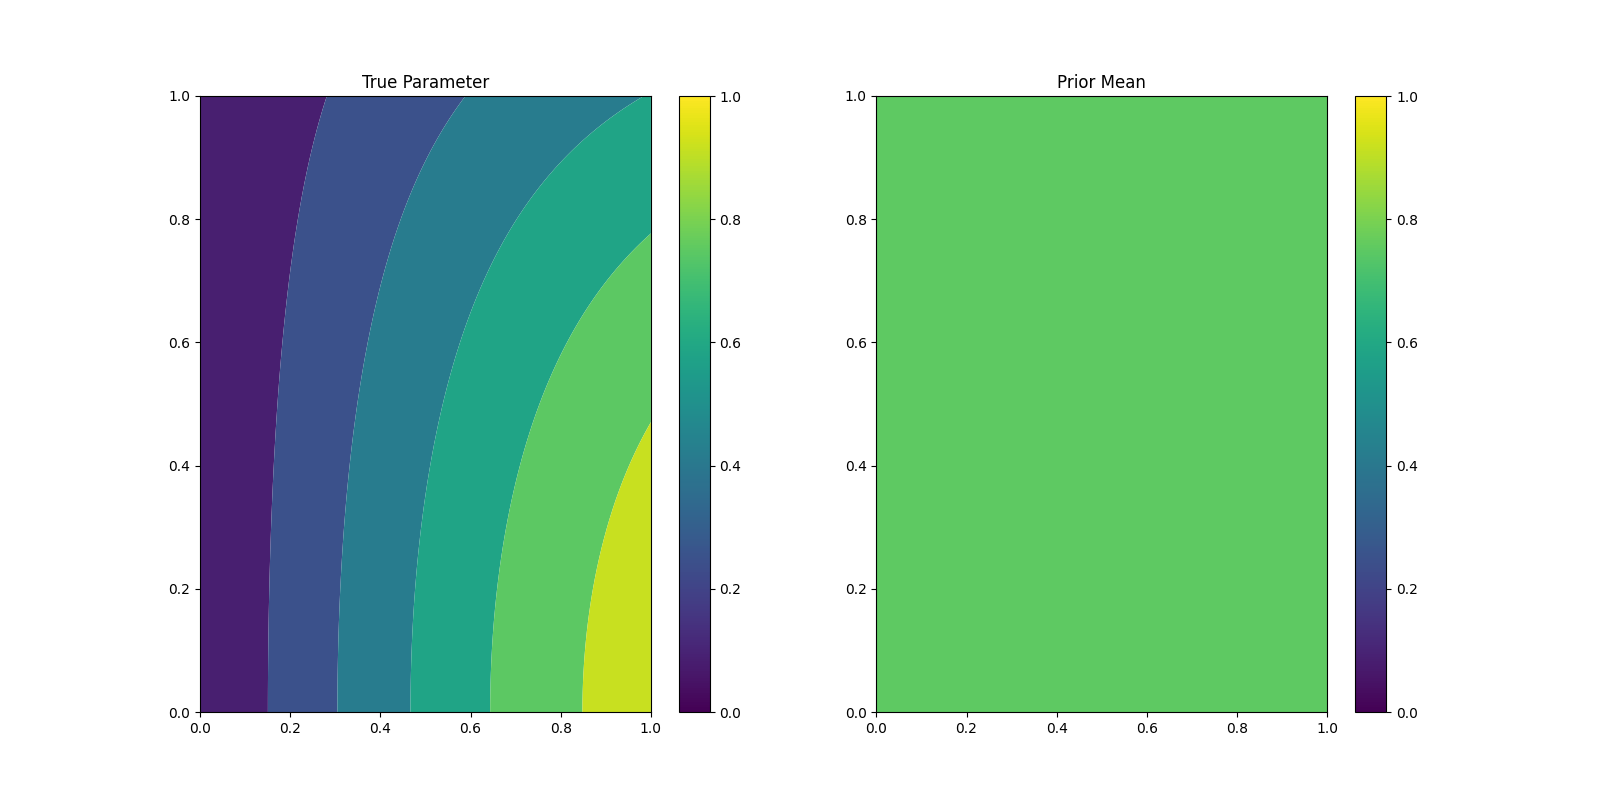
\includegraphics[width=1.0\textwidth]{figures/parameter.png}
        \caption{Variation of the true parameter and mean.}
        \label{figure:parameter}
        \end{figure}
    \item \textbf{Misfit}: \texttt{hIPPYfire} currently provides support for \texttt{ContinuousStateObservation}, which sets up the observation parameter $\mathcal{B}$. The observables which shall provide our input data are first generated by solving the forward problem by using the true parameter $\textbf{m}_{true}$
    \begin{lstlisting}[language=python]
        misfit = ContinuousStateObservation(Vh[STATE], ufl.dx, bcs=bc0)
        misfit.noise_variance = 1e-4
        utrue = pde.generate_state()
        x = [utrue, mtrue.vector(), None]
        pde.solveFwd(x[STATE], x)
        misfit.d.axpy(1., utrue)
        misfit.d.axpy(float(np.sqrt(misfit.noise_variance)), randomGen(Vh[STATE]).vector())
    \end{lstlisting}
    \begin{figure}[th]
        \centering
        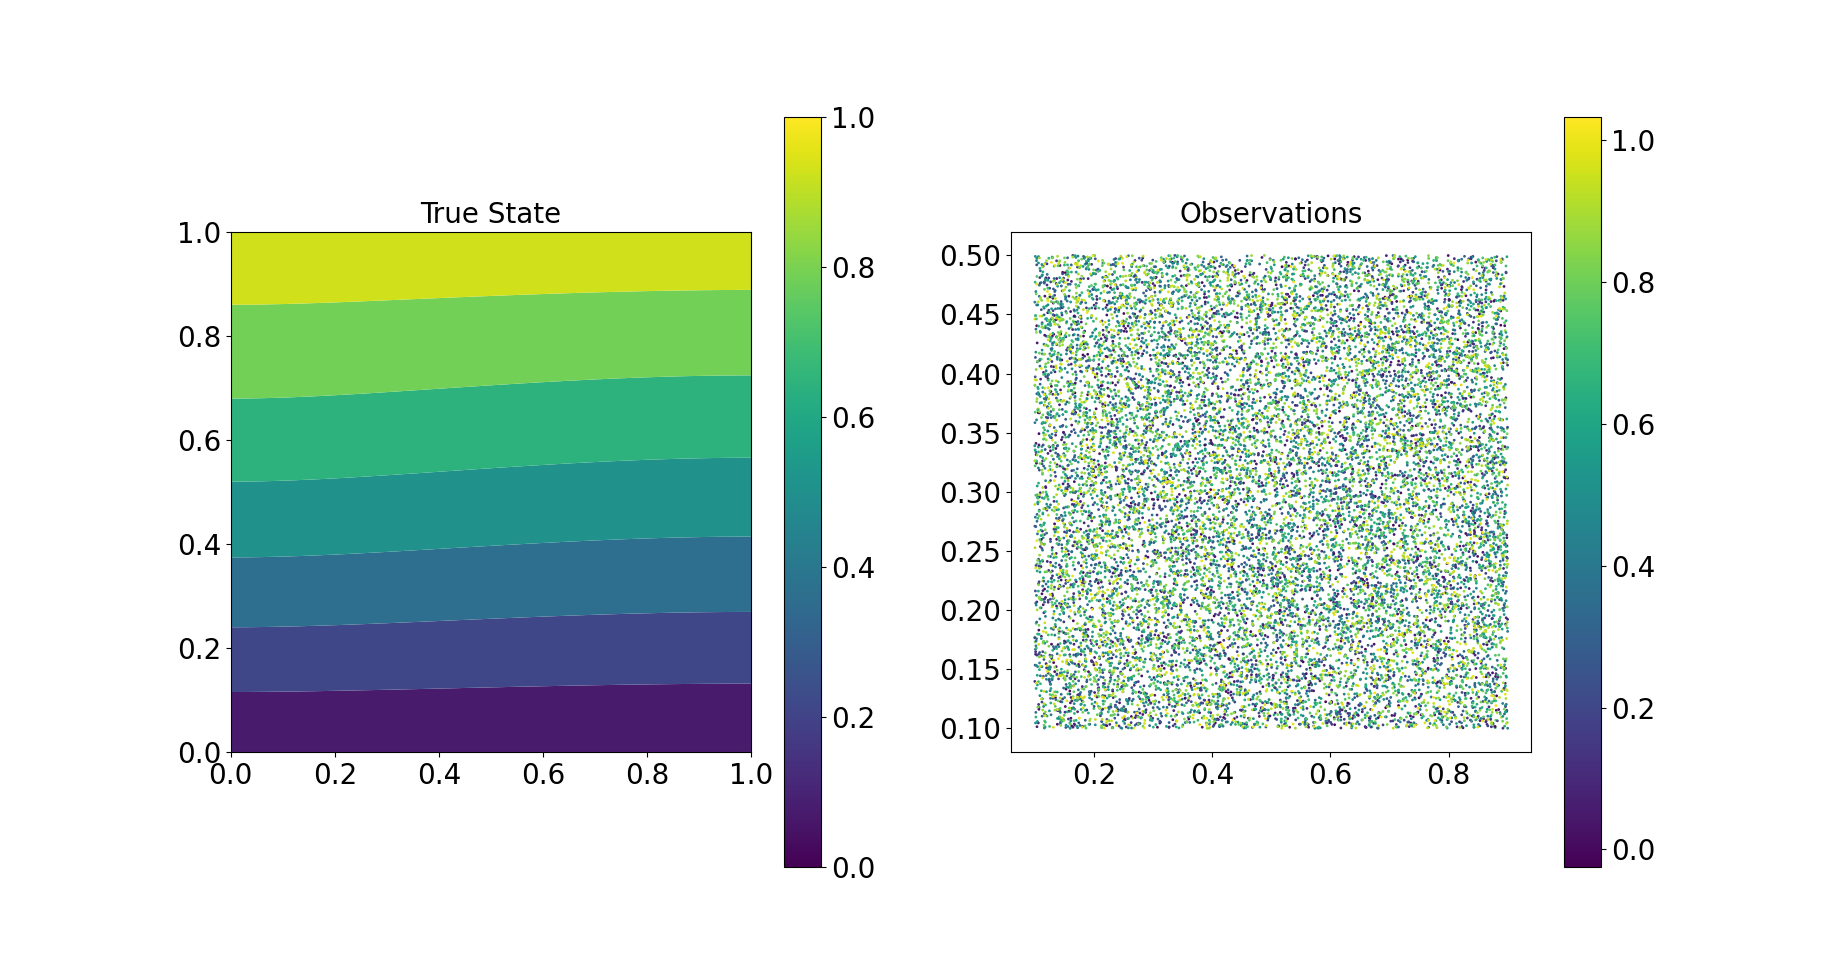
\includegraphics[width=1.0\textwidth]{figures/observations.png}
        \caption{Variation of the true state and the observations.}
        \label{figure:state}
    \end{figure}
    \item \textbf{Model}: The model, which is created by the \texttt{model} class, depends on three components---namely \texttt{PDEVariationalProblem}, \texttt{misfit}, and \texttt{prior}. The \texttt{PDEVariationalProblem} provides solutions for the forward and adjoint problems and incremental forward and adjoint problems. The \texttt{prior} applies the regularization operator to a vector, while the \texttt{misfit} computes the cost functional and partial derivatives with respect to the state and parameter variables.
    Forward finite differences are used to test the model through the \texttt{modelVerify} module.
    \begin{lstlisting}[language=python]
        model = Model(pde, pr, misfit)
        eps, err_grad, err_H = modelVerify(model, m0, misfit_only=False)
    \end{lstlisting}
    \begin{lstlisting}[language=bash]
        (yy, H xx) - (xx, H yy) =  0.0
    \end{lstlisting}
    \begin{figure}[th]
        \centering
        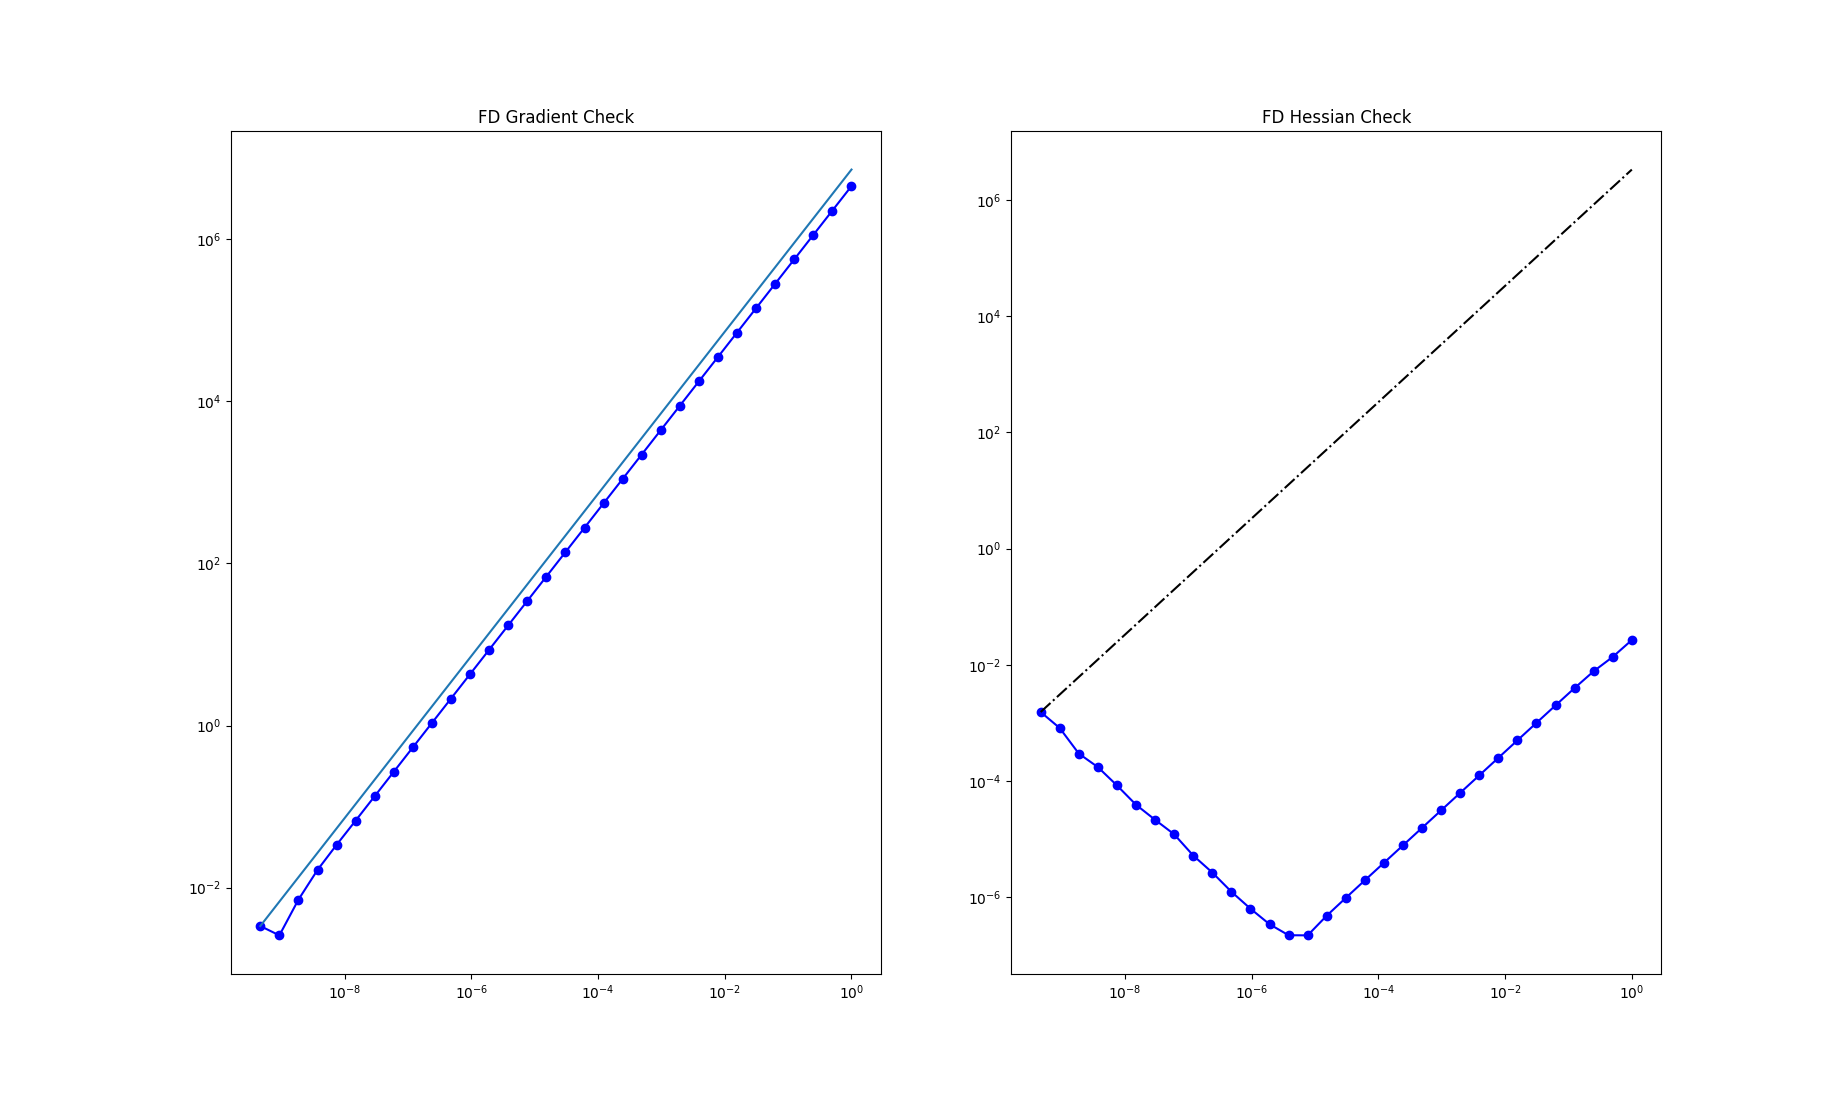
\includegraphics[width=1.0\textwidth]{figures/modelVerify.png}
        \caption{Gradient and Hessian Checks obtained from \texttt{modelVerify}}
        \label{figure:modelVerify}
    \end{figure}
    \hl{@Umberto, I am currently working to fix the aspect ratio of the gradient check plots. Should be fixed by EOD. The colorbars in the rest of the figures are slightly longer than the graph; I am rectifying those ASAP as well.}
    \item \textbf{MAP Point}: The Newton-CG method is used to compute the MAP point.
    \begin{lstlisting}[language=python]
        m = pr.mean.copy()
        solver = ReducedSpaceNewtonCG(model)
        solver.parameters["rel_tolerance"] = 1e-6
        solver.parameters["abs_tolerance"] = 1e-12
        solver.parameters["max_iter"]      = 25
        solver.parameters["GN_iter"] = 5
        solver.parameters["globalization"] = "LS"
        solver.parameters["LS"]["c_armijo"] = 1e-4
        x = solver.solve([None, m, None])
    \end{lstlisting}
    The following output was obtained:
    \begin{lstlisting}[language=bash]
        Relative/Absolute residual less than tol
Converged in  19  iterations with final norm  5.65259722013104e-08

It  cg_it cost            misfit          reg             (g,dm)          ||g||L2        alpha          tolcg         
1   1    9.452277e-01    8.990612e-01    4.616652e-02   -2.456844e+01   1.685316e+02   1.000000e+00   5.000000e-01
2   2    4.228824e-01    3.488744e-01    7.400803e-02   -1.043988e+00   1.715492e+01   1.000000e+00   3.190463e-01
3   5    4.027649e-01    3.196818e-01    8.308311e-02   -4.042007e-02   3.036538e+00   1.000000e+00   1.342297e-01
4   7    4.026241e-01    3.196381e-01    8.298594e-02   -3.009693e-04   2.404168e-01   1.000000e+00   3.776954e-02
5   7    4.026228e-01    3.196101e-01    8.301271e-02   -2.859017e-06   1.569884e-02   1.000000e+00   9.651461e-03
6   8    4.026228e-01    3.196134e-01    8.300935e-02   -4.118272e-08   8.007385e-04   1.000000e+00   2.179740e-03
5.941225051879883 Executiion time

Converged in  6  iterations.
Termination reason:  Norm of the gradient less than tolerance
Final gradient norm:  7.784347671669573e-06
Final cost:  0.40262278305284716
    \end{lstlisting}
    \begin{figure}[th]
        \centering
        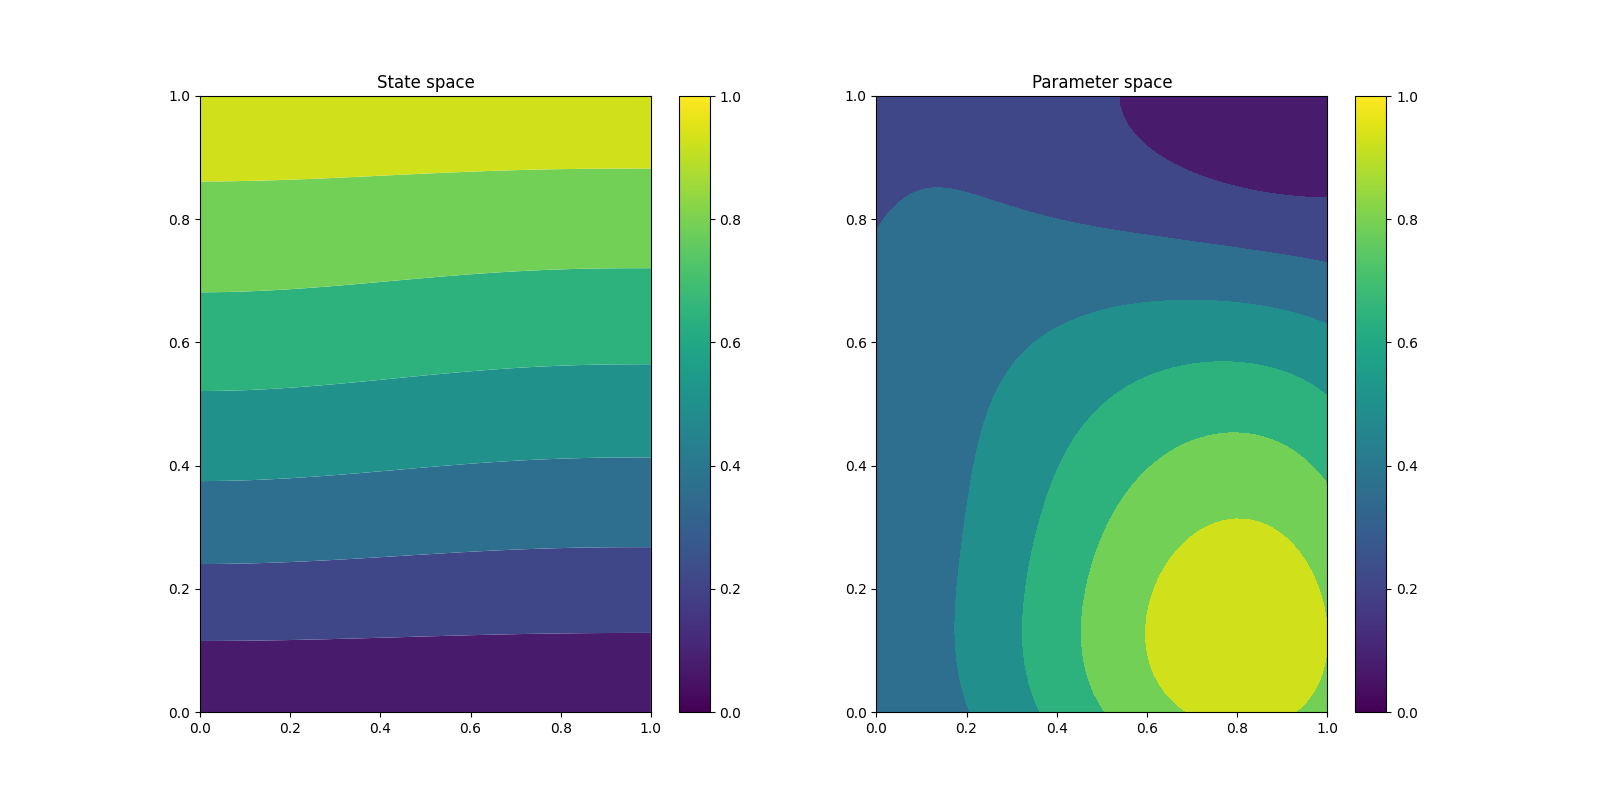
\includegraphics[width=1.0\textwidth]{figures/space.png}
        \caption{Contours of the state and parameter}
        \label{figure:space}
    \end{figure}
    A mesh independence study was conducted to establish that the convergence of the problem is observed for different sizes. The current sample assumes a uniform square mesh with 64 divisions. Experiments were conducted for mesh sizes of 128 and 256 divisions. Convergence was reported for 6--7 iterations for all mesh sizes. 
\end{itemize}